\setauthor{Antonio Kuvac}

Die erste und auch längste Phase dieses Projekts war die Planung. 
In der Planungsphase wurden verschiedenste Kreativitätstechniken angewandt und Dokumente, die für die Planung unerlässlich sind, erstellt.

\section{Projektpartnermeetings}
\setauthor{Antonio Kuvac}

Der Grundstein für diese Arbeit waren die abgehaltenen Meetings mit dem Projektpartner dieses Projekts. Bei den ersten Meetings wurde definiert, was die App können muss und wie die App auszusehen hat
um Missverständnisse im voraus zu behandeln und um sich ein Bild darüber zu machen, welche Anforderungen das Projekt hat und welche Herausforderungen zu bewältigen sind. 
Mit diesen Meetings wurde der Projektpartner auch auf aktuellen Stand gehalten und auftretende Probleme und Anmerkungen, 
die bei der Arbeit am Projekt entstanden sind, wurden besprochen und abgehandelt.

\section{Use-Case Diagramm}
\setauthor{Antonio Kuvac}

Ein Use Case Diagramm oder auch Anwendungsfalldiagramm ist ein Diagramm von Anwendungsfällen und ihren Beziehungen zu ihrer Umgebung und zu anderen Anwendungsfällen. 
Damit beschreibt es, welche Funktionen und Dienste ein System für einen Anwender bereitstellt.
Mit einem Use Case Diagramm werden weder die Abläufe des Systems beschrieben, 
noch die Reihenfolge der Funktionen oder Dienste dargestellt. 
Ein Anwendungsfalldiagramm visualisiert lediglich die Zusammenhänge zwischen einer Menge von Use Cases und den involvierten Akteuren. Damit eignet es sich sehr gut zur Anforderungsanalyse, also zur Ermittlung oder Verfeinerung von Anforderungen.
\pagebreak
\subsection{Elemente im Use-Case Diagramm}

Folgende Elemente sind in einem Use-Case Diagramm üblicherweise enthalten:
\begin{itemize}
    \item System: Das System ist an sich kein logisches Modellelement, sondern grenzt den Kontext ab. Das System wird durch eine Box im Diagramm dargestellt, in dem das System seine Funktionen und Dienste zur Verfügung stellt.
    \item Akteur: Der Akteur befindet sich außerhalb des Systems. Er wird als Strichmännchen gezeichnet und kann eine konkrete Person aber auch ein abstraktes Element wie zum Beispiel ein Sensor sein. Wird ein Akteur definiert, muss dieser auch immer mit mindestens einem Use Case in Verbindung stehen.
    \item Anwendungsfall: Ein Anwendungsfall wird meistens als Ellipse visualisiert. Ein Diagramm kann mehrere Anwendungsfälle besitzen. Ist ein Use Case nur durch andere Anwendungsfälle ausführbar, wird er als abstrakt bezeichnet.
    \item Beziehungen: Zwischen Akteuren und Anwendungsfällen oder zwischen Anwendungsfällen selbst bestehen Beziehungen. Sie werden meistens als Linien oder Pfeile zwischen den jeweiligen Objekten eingezeichnet.
    \item Notizen: Mit Notizen lassen sich Informationen hinzufügen, um das Verständnis zu erhöhen. Sie werden mit einem Rechteck dargestellt, dessen obere rechte Ecke eingeknickt ist. Eine gestichelte Linie verbindet die Notiz mit dem zu erklärenden Element.
    
    \end{itemize}
    \pagebreak
    \subsection{Verwendung des Use-Case Diagramms in der Diplomarbeit}

    Das Use Case Diagramm wurde verwendet um Klarheit über die Funktionen und den Akteuren zu schaffen und für Vergewisserung zu sorgen, dass keine wichtigen Verbindungen vergessen wurden.
    Am Ende der Planungsphase angelangt sieht das Use-Case Diagramm wie folgt aus:

    \begin{figure}[H]
        \centering
        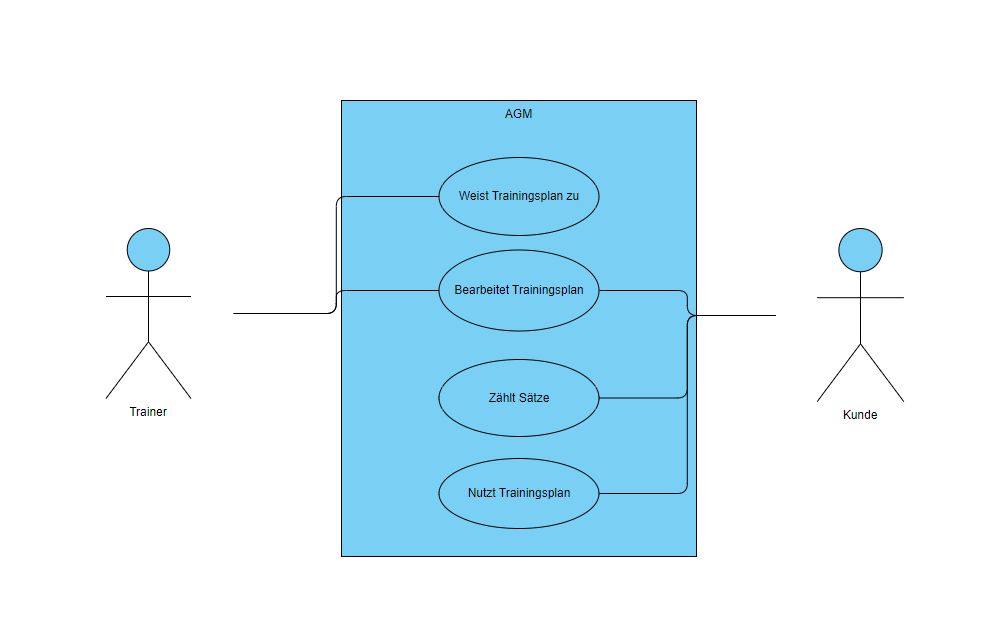
\includegraphics[scale=0.6]{pics/Use Case Diagramm.png}
        \caption{Use-Case Diagramm}
    \end{figure}
    